\let\negmedspace\undefined
\let\negthickspace\undefined
\documentclass[journal]{IEEEtran}
\usepackage[a5paper, margin=10mm, onecolumn]{geometry}
%\usepackage{lmodern} % Ensure lmodern is loaded for pdflatex
\usepackage{tfrupee} % Include tfrupee package

\setlength{\headheight}{1cm} % Set the height of the header box
\setlength{\headsep}{0mm}     % Set the distance between the header box and the top of the text

\usepackage{gvv-book}
\usepackage{gvv}
\usepackage{cite}
\usepackage{amsmath,amssymb,amsfonts,amsthm}
\usepackage{algorithmic}
\usepackage{graphicx}
\usepackage{textcomp}
\usepackage{xcolor}
\usepackage{txfonts}
\usepackage{listings}
\usepackage{enumitem}
\usepackage{mathtools}
\usepackage{gensymb}
\usepackage{comment}
\usepackage[breaklinks=true]{hyperref}
\usepackage{tkz-euclide} 
\usepackage{listings}
% \usepackage{gvv}                                        
\def\inputGnumericTable{}                                 
\usepackage[latin1]{inputenc}                                
\usepackage{color}                                            
\usepackage{array}                                            
\usepackage{longtable}                                       
\usepackage{calc}                                             
\usepackage{multirow}                                         
\usepackage{hhline}                                           
\usepackage{ifthen}                                           
\usepackage{lscape}
\begin{document}

\bibliographystyle{IEEEtran}
\vspace{3cm}

\title{1.10.11}
\author{EE25BTECH11053 - Surya Sri}
% \maketitle
% \newpage
% \bigskip
{\let\newpage\relax\maketitle}

\renewcommand{\thefigure}{\theenumi}
\renewcommand{\thetable}{\theenumi}
\setlength{\intextsep}{10pt} % Space between text and floats

\textbf{Question}:\\
Find a vector of magnitude 5 units, and parallel to the resultant of the vectors $\vec{a} = 2\hat{i} + 3\hat{j} - \hat{k}$ and $\vec{b} = \hat{i} - 2\hat{j} + \hat{k}$.


\bigskip
\textbf{Solution}:



Let the required vector be $\vec{R}$ ,

\begin{align}
    \vec{R} = k \frac{\vec{a} + \vec{b}}{\norm{\vec{a} + \vec{b}}}
\end{align}

  According to the question k = 5 ,
\begin{align}
     \vec{a} = \begin{pmatrix} 2 \\ 3 \\ -1 \end{pmatrix} 
 \end{align}
 \begin{align}
 \vec{b} = \begin{pmatrix} 1 \\ -2 \\ 1 \end{pmatrix} 
 \end{align}

\begin{align}
\vec{a} + \vec{b} = \begin{pmatrix} 3 \\ 1 \\ 0 \end{pmatrix}
\end{align}
So,
\begin{align}
\vec{p} = 5 \frac{\begin{pmatrix} 3 \\ 1 \\ 0 \end{pmatrix}}{\sqrt{3^2 + 1^2 + 0^2}} = \frac{5}{\sqrt{10}} \begin{pmatrix} 3 \\ 1 \\ 0 \end{pmatrix}
\end{align}


\begin{align}
\boxed{
\vec{p} = \frac{5}{\sqrt{10}}
\begin{pmatrix}
3 \\
1 \\
0
\end{pmatrix}
}
\end{align}




\begin{figure}[H]
\begin{center}
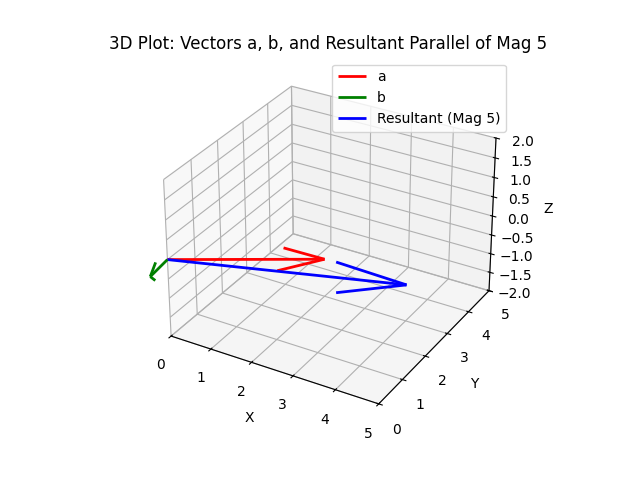
\includegraphics[width=0.75\columnwidth]{figs/graph.png}
\end{center}
\caption{}
\label{fig:Fig}
\end{figure}





\end{document}
